% Indicate the main file. Must go at the beginning of the file.
% !TEX root = ../main.tex

%----------------------------------------------------------------------------------------
% CHAPTER 4
%----------------------------------------------------------------------------------------

\chapter{Survey}

\label{Chapter4} % For referencing the chapter elsewhere, use \ref{Chapter2} 

In order to gain insight into potential adoption of these technologies, a survey was conducted among software engineering professionals. In total, 48 responses were collected from various teams and companies across diverse engineering domains. The survey questions were organized into four main themes: participant demographics, role-based information presentation in documents, decision logs within a mirrored approach, and infrastructure as code. The final section of the survey includes a further optional question. This is designed to elicit participants’ interpretations of the potential combinations of tooling. It is hoped that the responses to this question will help identify solutions that work well together and may even enhance the implementation and maintenance of these solutions.
The questions and information provided in the survey are given in Appendix A. The questions were developed with a specific aim in mind: namely, to validate the different tools in order to improve the collaboration and productivity within a SCRUM team. In addition, the questions seek to identify the problems and weaknesses of the real process, and thus provide a basis for the formulation of better approaches and solutions that are both resourceful and effective and accepted by the whole team.


\section{Demographics}


\section{Role Based Information Highlighting in Documents}

\subsection{Do you usually get overwhelmed by the amount of information when reading documentations?}
As we can see in the figure \ref{fig:results:decisions:1} 34 \% voted more than eight on the scala 


\begin{figure}[h!]
\centering
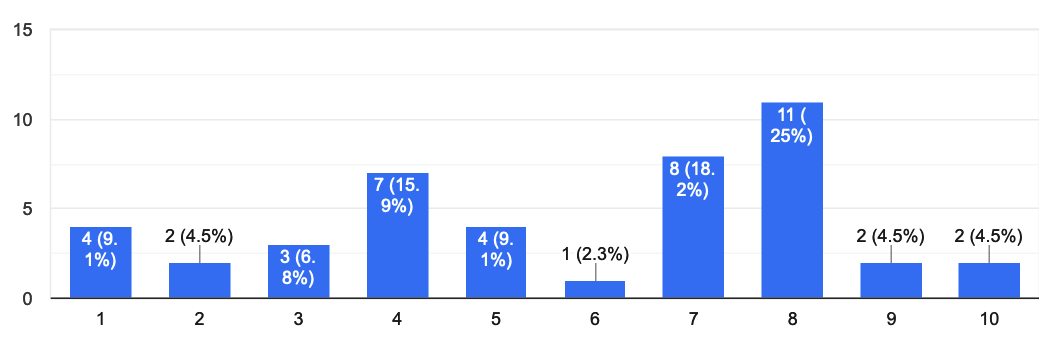
\includegraphics[width=\linewidth]{Images/Survey/documents_1.png}
\caption{Results for - Do you usually get overwhelmed by the amount of information when reading documentations?}
\label{fig:results:highlighting:1}
\end{figure}

\subsection{How satisfying would it be to have the information that is most important to you highlighted for you?}
Lorem ipsum dolor sit amet, consetetur sadipscing elitr, sed diam nonumy eirmod tempor invidunt ut labore et dolore magna aliquyam erat, sed diam voluptua. At vero eos et accusam et justo duo dolores et ea rebum. Stet clita kasd gubergren, no sea takimata sanctus est Lorem ipsum dolor sit amet. Lorem ipsum dolor sit amet, consetetur sadipscing elitr, sed diam nonumy eirmod tempor invidunt ut labore et dolore magna aliquyam erat, sed diam voluptua. At vero eos et accusam et justo duo dolores et ea rebum. Stet clita kasd gubergren, no sea takimata sanctus est Lorem ipsum dolor sit amet.
\begin{figure}[h!]
\centering
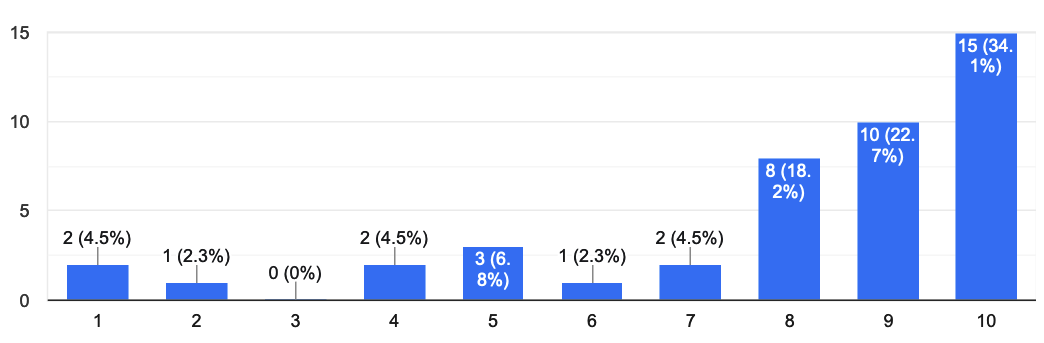
\includegraphics[width=\linewidth]{Images/Survey/documents_2.png}
\caption{Results for - How satisfying would it be to have the information that is most important to you highlighted for you?}
\label{fig:results:highlighting:2}
\end{figure}


\subsection{How easy do you think it would be to use AI to automate the highlighting of information based on a viewer's role selection?}
Lorem ipsum dolor sit amet, consetetur sadipscing elitr, sed diam nonumy eirmod tempor invidunt ut labore et dolore magna aliquyam erat, sed diam voluptua. At vero eos et accusam et justo duo dolores et ea rebum. Stet clita kasd gubergren, no sea takimata sanctus est Lorem ipsum dolor sit amet. Lorem ipsum dolor sit amet, consetetur sadipscing elitr, sed diam nonumy eirmod tempor invidunt ut labore et dolore magna aliquyam erat, sed diam voluptua. At vero eos et accusam et justo duo dolores et ea rebum. Stet clita kasd gubergren, no sea takimata sanctus est Lorem ipsum dolor sit amet.
\begin{figure}[h!]
\centering
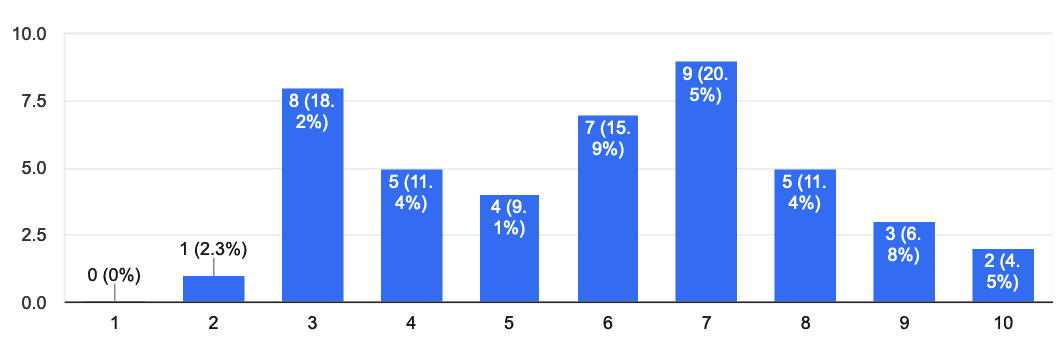
\includegraphics[width=\linewidth]{Images/Survey/documents_3.png}
\caption{Results for - How easy do you think it would be to use AI to automate the highlighting of information based on a viewer's role selection?}
\label{fig:results:highlighting:3}
\end{figure}

\subsection{How much better do you think this approach of highlighting just the right information is than having separate pages for different roles?}
Lorem ipsum dolor sit amet, consetetur sadipscing elitr, sed diam nonumy eirmod tempor invidunt ut labore et dolore magna aliquyam erat, sed diam voluptua. At vero eos et accusam et justo duo dolores et ea rebum. Stet clita kasd gubergren, no sea takimata sanctus est Lorem ipsum dolor sit amet. Lorem ipsum dolor sit amet, consetetur sadipscing elitr, sed diam nonumy eirmod tempor invidunt ut labore et dolore magna aliquyam erat, sed diam voluptua. At vero eos et accusam et justo duo dolores et ea rebum. Stet clita kasd gubergren, no sea takimata sanctus est Lorem ipsum dolor sit amet.
\begin{figure}[h!]
\centering
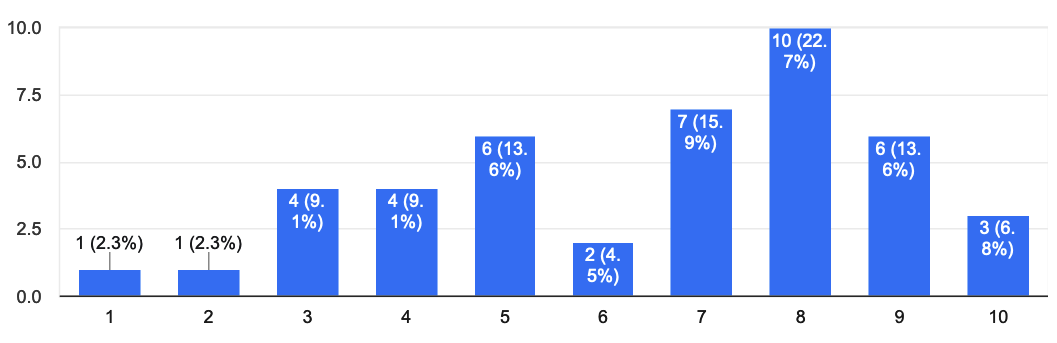
\includegraphics[width=\linewidth]{Images/Survey/documents_4.png}
\caption{Results for - How easy do you think it would be to use AI to automate the highlighting of information based on a viewer's role selection?}
\label{fig:results:highlighting:4}
\end{figure}

\subsection{In your personal experience, do you see people using more text or screenshots to document information?}
Lorem ipsum dolor sit amet, consetetur sadipscing elitr, sed diam nonumy eirmod tempor invidunt ut labore et dolore magna aliquyam erat, sed diam voluptua. At vero eos et accusam et justo duo dolores et ea rebum. Stet clita kasd gubergren, no sea takimata sanctus est Lorem ipsum dolor sit amet. Lorem ipsum dolor sit amet, consetetur sadipscing elitr, sed diam nonumy eirmod tempor invidunt ut labore et dolore magna aliquyam erat, sed diam voluptua. At vero eos et accusam et justo duo dolores et ea rebum. Stet clita kasd gubergren, no sea takimata sanctus est Lorem ipsum dolor sit amet.
\begin{figure}[h!]
\centering
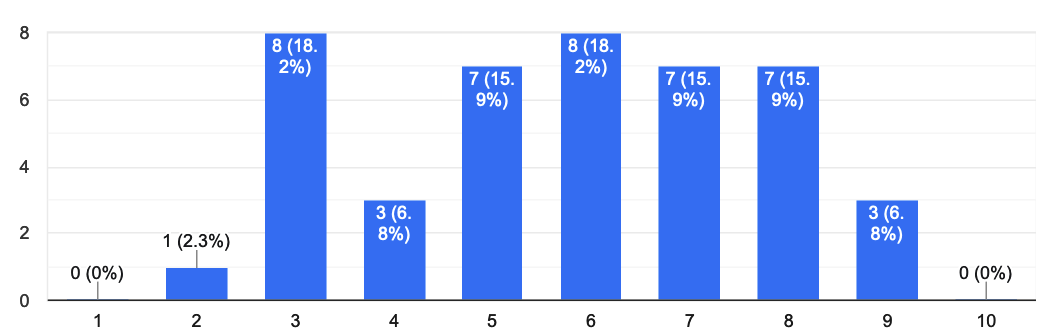
\includegraphics[width=\linewidth]{Images/Survey/documents_5.png}
\caption{Results for - In your personal experience, do you see people using more text or screenshots to document information?}
\label{fig:results:highlighting:5}
\end{figure}

\section{Decision Logs Within a Mirrored Approach}

\subsection{How important do you think it is to have a record of decisions and an up-to-date record of decisions?}
Lorem ipsum dolor sit amet, consetetur sadipscing elitr, sed diam nonumy eirmod tempor invidunt ut labore et dolore magna aliquyam erat, sed diam voluptua. At vero eos et accusam et justo duo dolores et ea rebum. Stet clita kasd gubergren, no sea takimata sanctus est Lorem ipsum dolor sit amet. Lorem ipsum dolor sit amet, consetetur sadipscing elitr, sed diam nonumy eirmod tempor invidunt ut labore et dolore magna aliquyam erat, sed diam voluptua. At vero eos et accusam et justo duo dolores et ea rebum. Stet clita kasd gubergren, no sea takimata sanctus est Lorem ipsum dolor sit amet.
\begin{figure}[h!]
\centering
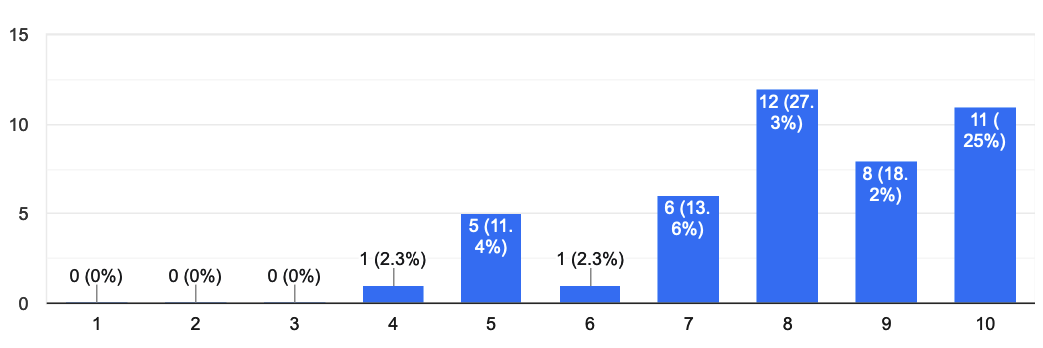
\includegraphics[width=\linewidth]{Images/Survey/decisions_1.png}
\caption{Results for - How important do you think it is to have a record of decisions and an up-to-date record of decisions?}
\label{fig:results:decisions:1}
\end{figure}

\subsection{Did the decision logs you've seen so far contain the most up-to-date information, were they properly formatted and did they make sense?}
Lorem ipsum dolor sit amet, consetetur sadipscing elitr, sed diam nonumy eirmod tempor invidunt ut labore et dolore magna aliquyam erat, sed diam voluptua. At vero eos et accusam et justo duo dolores et ea rebum. Stet clita kasd gubergren, no sea takimata sanctus est Lorem ipsum dolor sit amet. Lorem ipsum dolor sit amet, consetetur sadipscing elitr, sed diam nonumy eirmod tempor invidunt ut labore et dolore magna aliquyam erat, sed diam voluptua. At vero eos et accusam et justo duo dolores et ea rebum. Stet clita kasd gubergren, no sea takimata sanctus est Lorem ipsum dolor sit amet.
\begin{figure}[h!]
\centering
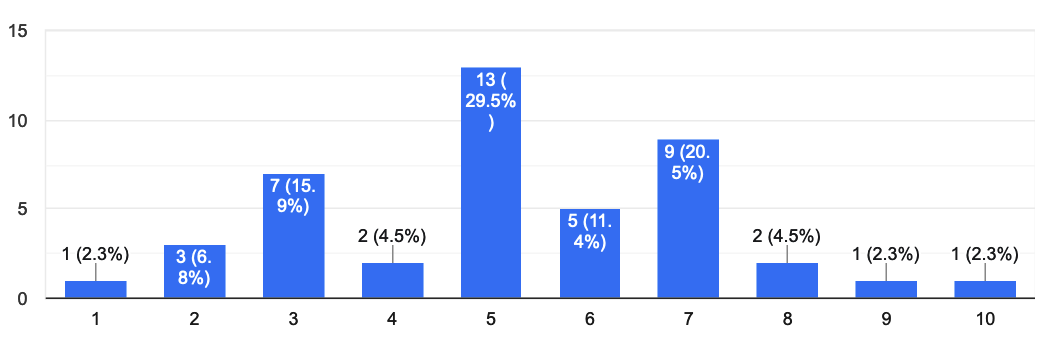
\includegraphics[width=\linewidth]{Images/Survey/decisions_2.png}
\caption{Results for - Did the decision logs you've seen so far contain the most up-to-date information, were they properly formatted and did they make sense?}
\label{fig:results:decisions:2}
\end{figure}

\subsection{How do you think the decision logs would benefit from being part of the relevant code base, rather than a separate document, in terms of being up to date?}
Lorem ipsum dolor sit amet, consetetur sadipscing elitr, sed diam nonumy eirmod tempor invidunt ut labore et dolore magna aliquyam erat, sed diam voluptua. At vero eos et accusam et justo duo dolores et ea rebum. Stet clita kasd gubergren, no sea takimata sanctus est Lorem ipsum dolor sit amet. Lorem ipsum dolor sit amet, consetetur sadipscing elitr, sed diam nonumy eirmod tempor invidunt ut labore et dolore magna aliquyam erat, sed diam voluptua. At vero eos et accusam et justo duo dolores et ea rebum. Stet clita kasd gubergren, no sea takimata sanctus est Lorem ipsum dolor sit amet.
\begin{figure}[h!]
\centering
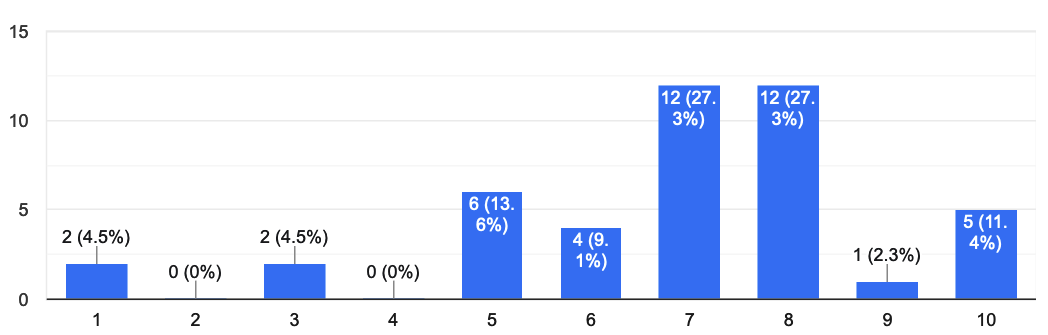
\includegraphics[width=\linewidth]{Images/Survey/decisions_3.png}
\caption{Results for - How do you think the decision logs would benefit from being part of the relevant code base, rather than a separate document, in terms of being up to date?}
\label{fig:results:decisions:3}
\end{figure}

\subsection{How important do you think it is, if the decision logs are in the associated codebase, to still keep them in a document accessible to "non-developers"?}
Lorem ipsum dolor sit amet, consetetur sadipscing elitr, sed diam nonumy eirmod tempor invidunt ut labore et dolore magna aliquyam erat, sed diam voluptua. At vero eos et accusam et justo duo dolores et ea rebum. Stet clita kasd gubergren, no sea takimata sanctus est Lorem ipsum dolor sit amet. Lorem ipsum dolor sit amet, consetetur sadipscing elitr, sed diam nonumy eirmod tempor invidunt ut labore et dolore magna aliquyam erat, sed diam voluptua. At vero eos et accusam et justo duo dolores et ea rebum. Stet clita kasd gubergren, no sea takimata sanctus est Lorem ipsum dolor sit amet.
\begin{figure}[h!]
\centering
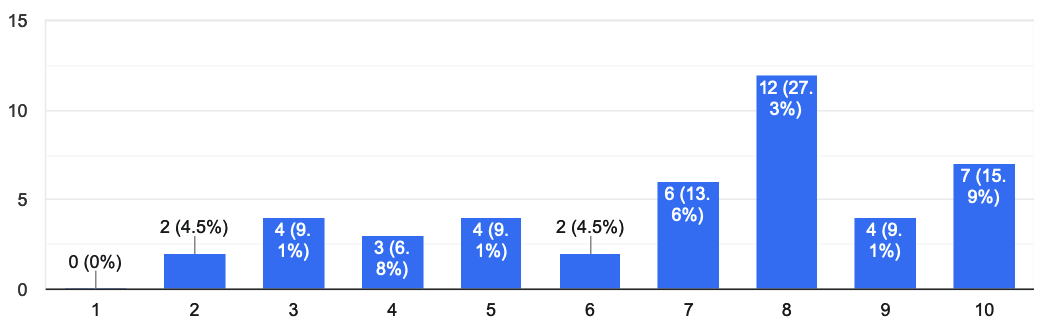
\includegraphics[width=\linewidth]{Images/Survey/decisions_4.png}
\caption{Results for - How important do you think it is, if the decision logs are in the associated codebase, to still keep them in a document accessible to "non-developers"?}
\label{fig:results:decisions:4}
\end{figure}


\subsection{How easy do you think it would be to use tools to automate the mirroring of decisions into a separate document accessible to everyone?}
Lorem ipsum dolor sit amet, consetetur sadipscing elitr, sed diam nonumy eirmod tempor invidunt ut labore et dolore magna aliquyam erat, sed diam voluptua. At vero eos et accusam et justo duo dolores et ea rebum. Stet clita kasd gubergren, no sea takimata sanctus est Lorem ipsum dolor sit amet. Lorem ipsum dolor sit amet, consetetur sadipscing elitr, sed diam nonumy eirmod tempor invidunt ut labore et dolore magna aliquyam erat, sed diam voluptua. At vero eos et accusam et justo duo dolores et ea rebum. Stet clita kasd gubergren, no sea takimata sanctus est Lorem ipsum dolor sit amet.
\begin{figure}[h!]
\centering
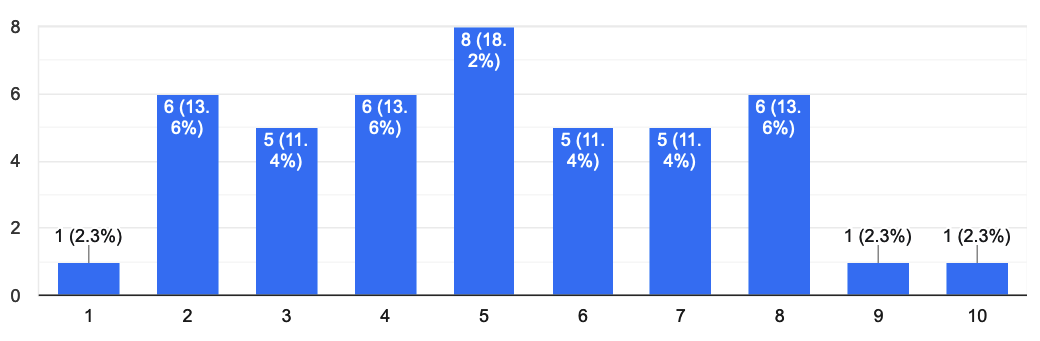
\includegraphics[width=\linewidth]{Images/Survey/decisions_5.png}
\caption{Results for - How easy do you think it would be to use tools to automate the mirroring of decisions into a separate document accessible to everyone?}
\label{fig:results:decisions:5}
\end{figure}


\section{Infrastructure As Code}

\subsection{In your current software project, how much do you know about how deployments and architectures work?}
Lorem ipsum dolor sit amet, consetetur sadipscing elitr, sed diam nonumy eirmod tempor invidunt ut labore et dolore magna aliquyam erat, sed diam voluptua. At vero eos et accusam et justo duo dolores et ea rebum. Stet clita kasd gubergren, no sea takimata sanctus est Lorem ipsum dolor sit amet. Lorem ipsum dolor sit amet, consetetur sadipscing elitr, sed diam nonumy eirmod tempor invidunt ut labore et dolore magna aliquyam erat, sed diam voluptua. At vero eos et accusam et justo duo dolores et ea rebum. Stet clita kasd gubergren, no sea takimata sanctus est Lorem ipsum dolor sit amet.
\begin{figure}[h!]
\centering
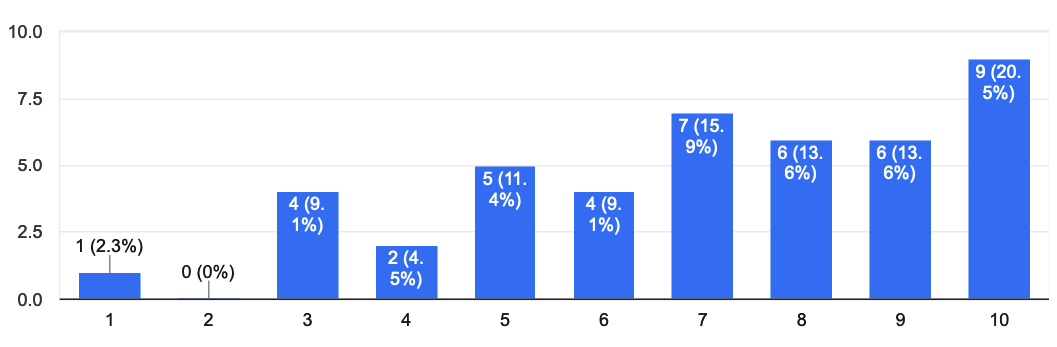
\includegraphics[width=\linewidth]{Images/Survey/iac_1.png}
\caption{In your current software project, how much do you know about how deployments and architectures work?}
\label{fig:results:iac:1}
\end{figure}


\subsection{How familiar are you with the concept of Infrastructure as Code (IaC) and its benefits?}
Lorem ipsum dolor sit amet, consetetur sadipscing elitr, sed diam nonumy eirmod tempor invidunt ut labore et dolore magna aliquyam erat, sed diam voluptua. At vero eos et accusam et justo duo dolores et ea rebum. Stet clita kasd gubergren, no sea takimata sanctus est Lorem ipsum dolor sit amet. Lorem ipsum dolor sit amet, consetetur sadipscing elitr, sed diam nonumy eirmod tempor invidunt ut labore et dolore magna aliquyam erat, sed diam voluptua. At vero eos et accusam et justo duo dolores et ea rebum. Stet clita kasd gubergren, no sea takimata sanctus est Lorem ipsum dolor sit amet.
\begin{figure}[h!]
\centering
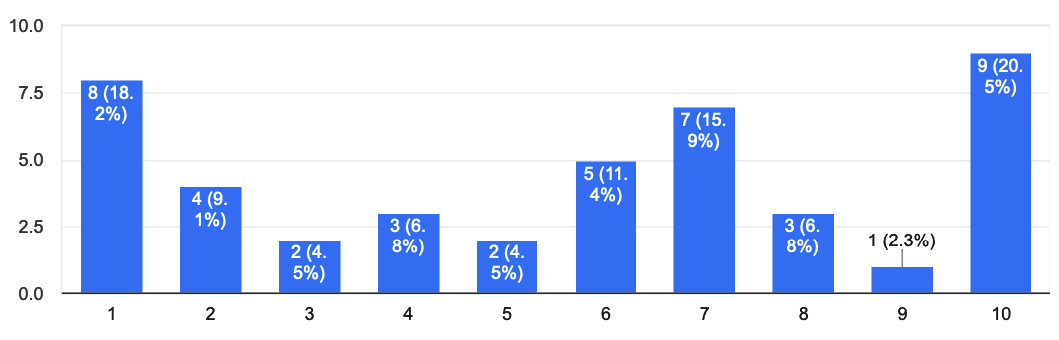
\includegraphics[width=\linewidth]{Images/Survey/iac_2.png}
\caption{How familiar are you with the concept of Infrastructure as Code (IaC) and its benefits?}
\label{fig:results:iac:2}
\end{figure}

\subsection{To what extent do you agree that IaC helps in fostering a sense of shared responsibility among development team members?}
Lorem ipsum dolor sit amet, consetetur sadipscing elitr, sed diam nonumy eirmod tempor invidunt ut labore et dolore magna aliquyam erat, sed diam voluptua. At vero eos et accusam et justo duo dolores et ea rebum. Stet clita kasd gubergren, no sea takimata sanctus est Lorem ipsum dolor sit amet. Lorem ipsum dolor sit amet, consetetur sadipscing elitr, sed diam nonumy eirmod tempor invidunt ut labore et dolore magna aliquyam erat, sed diam voluptua. At vero eos et accusam et justo duo dolores et ea rebum. Stet clita kasd gubergren, no sea takimata sanctus est Lorem ipsum dolor sit amet.
\begin{figure}[h!]
\centering
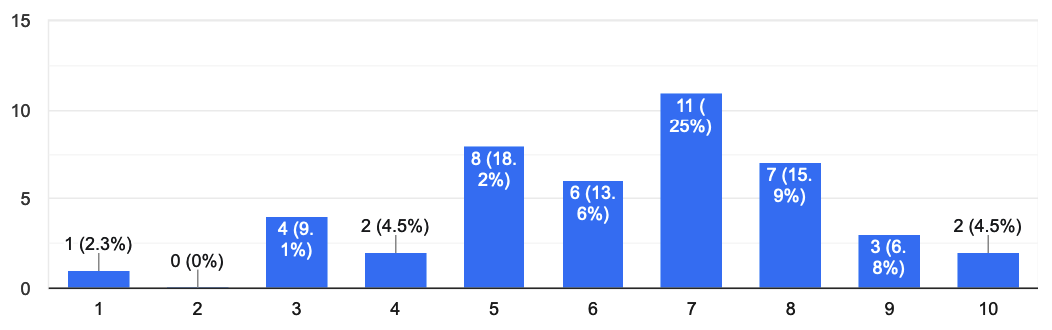
\includegraphics[width=\linewidth]{Images/Survey/iac_3.png}
\caption{To what extent do you agree that IaC helps in fostering a sense of shared responsibility among development team members?}
\label{fig:results:iac:3}
\end{figure}

\subsection{What are the biggest challenges or limitations you have faced when implementing IaC in your projects?}


\section{Summary}

\subsection{In your opinion, what combination of techniques would be the most effective?}


%----------------------------------------------------------------------------------------